\documentclass[11pt]{article}

% Change "review" to "final" to generate the final (sometimes called camera-ready) version.
% Change to "preprint" to generate a non-anonymous version with page numbers.
\usepackage[review]{acl}

% Standard package includes
\usepackage{times}
\usepackage{latexsym}

% For proper rendering and hyphenation of words containing Latin characters (including in bib files)
\usepackage[T1]{fontenc}
% For Vietnamese characters
% \usepackage[T5]{fontenc}
% See https://www.latex-project.org/help/documentation/encguide.pdf for other character sets

% This assumes your files are encoded as UTF8
\usepackage[utf8]{inputenc}

% This is not strictly necessary, and may be commented out,
% but it will improve the layout of the manuscript,
% and will typically save some space.
\usepackage{microtype}

% This is also not strictly necessary, and may be commented out.
% However, it will improve the aesthetics of text in
% the typewriter font.
\usepackage{inconsolata}

%Including images in your LaTeX document requires adding
%additional package(s)
\usepackage{graphicx}



%\usepackage[square,numbers]{natbib}



\usepackage{hyperref}       % hyperlinks
\usepackage{url}            % simple URL typesetting
\usepackage{booktabs}       % professional-quality tables
\usepackage{amsfonts}       % blackboard math symbols
\usepackage{amsmath}       
\usepackage{nicefrac}       % compact symbols for 1/2, etc.
\usepackage{microtype}      % microtypography
\usepackage{xcolor}         % colors


\usepackage[inline]{enumitem}
\usepackage{makecell}
\usepackage{fancyhdr}       % header
\usepackage{subcaption}
\usepackage{mdframed}
\usepackage{comment}
\usepackage{tabularx}
\usepackage{caption}
\usepackage{placeins}
\usepackage{float}
\usepackage{array} % for centering column content  
\usepackage{wrapfig}
\usepackage{cleveref}
\usepackage{multirow}
\usepackage{algorithm}
\usepackage{algorithmic}
\usepackage{listings}
\usepackage{atbeginend}
%\usepackage{pifont}

\newenvironment{packed_enum}{
\begin{enumerate}
	\setlength{\itemsep}{1pt}
	\setlength{\parskip}{0pt}
	\setlength{\parsep}{0pt}
}{\end{enumerate}}

\newenvironment{packed_item}{
\begin{itemize}
	\setlength{\itemsep}{1pt}
	\setlength{\parskip}{0pt}
	\setlength{\parsep}{0pt}
}{\end{itemize}}

\newenvironment{packed_description}{
\begin{description}
	\setlength{\itemsep}{1pt}
	\setlength{\parskip}{0pt}
	\setlength{\parsep}{0pt}
}{\end{description}}

\AfterBegin{packed_enum}{\vspace{-0.7em}}
\AfterEnd{packed_enum}{\vspace{-0.7em}}
\AfterBegin{packed_item}{\vspace{-0.7em}}
\AfterEnd{packed_item}{\vspace{-0.7em}}
\AfterBegin{packed_description}{\vspace{-0.7em}}
\AfterEnd{packed_description}{\vspace{-0.7em}}

\AfterBegin{quote}{\vspace{-0.7em}}
\AfterEnd{quote}{\vspace{-0.7em}}

\lstdefinelanguage{json}{
basicstyle=\ttfamily,
numbers=left,
numberstyle=\tiny\color{gray},
stepnumber=1,
numbersep=8pt,
showstringspaces=false,
breaklines=true,
%	frame=lines,
%	backgroundcolor=\color{lightgray},
literate=
*{0}{{{\color{blue}0}}}{1}
{1}{{{\color{blue}1}}}{1}
{2}{{{\color{blue}2}}}{1}
{3}{{{\color{blue}3}}}{1}
{4}{{{\color{blue}4}}}{1}
{5}{{{\color{blue}5}}}{1}
{6}{{{\color{blue}6}}}{1}
{7}{{{\color{blue}7}}}{1}
{8}{{{\color{blue}8}}}{1}
{9}{{{\color{blue}9}}}{1}
{:}{{{\color{red}:}}}{1}
{,}{{{\color{red},}}}{1}
{\{}{{{\color{orange}\{}}}{1}
{\}}{{{\color{orange}\}}}}{1}
{[}{{{\color{orange}[}}}{1}
{]}{{{\color{orange}]}}}{1},
}

\lstdefinelanguage{txt}{
basicstyle=\ttfamily,
numbers=left,
numberstyle=\tiny\color{gray},
stepnumber=1,
numbersep=8pt,
showstringspaces=false,
breaklines=true,
%	frame=lines,
%	backgroundcolor=\color{lightgray},
}



%
% These are are recommended to typeset listings but not required. See the subsubsection on listing. Remove this block if you don't have listings in your paper.
\usepackage{newfloat}
%\DeclareCaptionStyle{ruled}{labelfont=normalfont,labelsep=colon,strut=off} % DO NOT CHANGE THIS
\lstset{%
basicstyle={\footnotesize\ttfamily},% footnotesize acceptable for monospace
numbers=left,numberstyle=\footnotesize,xleftmargin=2em,% show line numbers, remove this entire line if you don't want the numbers.
aboveskip=0pt,belowskip=0pt,%
showstringspaces=false,tabsize=2,breaklines=true}
\floatstyle{ruled}
\newfloat{listing}{tb}{lst}{}
\floatname{listing}{Listing}
%
% Keep the \pdfinfo as shown here. There's no need
% for you to add the /Title and /Author tags.
\pdfinfo{
/TemplateVersion (2024.1)
}

\setcounter{secnumdepth}{3} %May be changed to 1 or 2 if section numbers are desired.

%Header
\pagestyle{fancy}
\thispagestyle{empty}
\rhead{ \textit{ }} 

% Title

%\title{Evaluating LM Accuracy Uplift From Rewriting Questions to Remove Ambiguities}
%\title{Evaluating LM Accuracy Uplift: Using Answer Free Context to Double gpt-oss-20b Performance on a subset of HLE}
\title{LM Accuracy Uplift: Using Answer-Free Context Information to Double gpt-oss-20b Performance on a subset of HLE}
%\title{Squeezing All Improvement From Your Context: QA Accuracy Uplift Even When the Context Doens't Surface the Answer}


\author{%
	Michael Majurski$^{12*}$ \quad Cynthia Matuszek$^{2}$\\
	$^1$National Institute of Standards and Technology \quad $^2$University of Maryland Baltimore County\\
	\texttt{michael.majurski@nist.gov}\\
	\texttt{cmat@umbc.edu}\\
}





\begin{document}

\maketitle


\begin{abstract}
Language Models (LMs) continue to advance, improving capability, response quality, and coherence. 
Given Internet-scale training datasets, LMs have likely encountered much of what users may ask them to generate in some form during their training. 
A plethora of evaluation benchmarks have been constructed to assess model quality, response appropriateness, and reasoning capabilities. 
However, the human effort required for benchmark construction is rapidly being outpaced by the size and scope of the models under evaluation.
Having humans build a benchmark for every possible domain of interest is impractical.
Therefore, we propose a methodology for automating the construction of fact-based synthetic data model evaluations grounded in document populations.
This work leverages the same LMs to evaluate domain-specific knowledge automatically, using only grounding documents (e.g., a textbook) as input.
This synthetic data benchmarking approach corresponds well with human curated questions producing an ensemble Spearman ranking correlation of $0.91$ and a benchmark evaluation Pearson accuracy correlation of $0.74$ (model specific $0.82$).
This novel approach supports generating both multiple choice and open-ended synthetic data questions to gain diagnostic insight of LM capability.
We apply this methodology to evaluate model performance on three recent documents (two post LM knowledge cutoff), discovering a surprisingly strong performance from Gemma-3 models on open-ended questions.
% TODO fill in before final camera ready
%	Code is available at \url{https://github.com/mmajurski/grounded-synth-lm-benchmark}
\end{abstract}



\section{Introduction}

\begin{figure}[t!]
	%	\vspace*{-1.0em}
	\centering
	\includegraphics[width=1.0\columnwidth]{figs/fig1.jpg}
	\vspace{-1.5em}
	\caption{lifehas3rules
		Synthetic evaluation pipeline: (1) users curate grounding documents, (2) LMs generate domain-specific questions, (3) model responses are evaluated. }
	\label{fig:evaluation-framework}
	\vspace{-1em}   
\end{figure}


\begin{figure}[b!]
	\vspace*{-1.0em}
	\centering
	\includegraphics[width=1.0\columnwidth]{figs/gpt120b-afc_hle.pdf}
	\vspace{-1.5em}
	\caption{Humanities Last Exam (HLE) benchmark evaluation accuracy using the original reference questions (x-axis) compared to the reformated generated by model ensemble demonstrating reasonable correlation between human and synthetic evaluation}
	\label{fig:hle-ref-vs-reformat}
%	\vspace{-1em}   
\end{figure}

The ongoing explosion of Language Model (LM) capability is largely a consequence of scaling laws, which have demonstrated a relationships between performance and parameter count, dataset size, and compute. 
%The rise of large models resulted in emergent capabilities such as few-shot and in-context learning.
This growth has opened a widening chasm between what modern LMs can do and how we measure their abilities.
Specifically, with AI systems targeting professional workflows, new types of evaluation is required to characterize LM capability when grounded in document populations.
LMs possess considerable general knowledge; but are inherently weaker with domain-specific and proprietary information. 
For enterprise applications with internal corporate knowledge management the generalized information contained within a pre-trained LM is insufficient. 
These domains require access to private, specialized, and often confidential data that is not part of any public training corpus. 
The current approach to solving this involve retrieval systems which dynamically fetch relevant context for the LM~\cite{NEURIPS2024_db93ccb6}.
Evaluation of RAG systems focuses heavily on ranking quality and retrieval performance~\cite{yang2024crag,NEURIPS2024_27245589}.



\begin{figure}[h!]
	\vspace*{-1.0em}
	\centering
	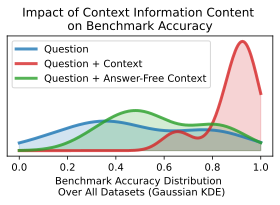
\includegraphics[width=0.9\columnwidth]{figs/impact_of_context_gpt-oss-120b.pdf}
	\vspace{-0.8em}
	\caption{The context information presented to the LM answering questions has a drastic impact on performance. When RAG-type systems correctly surface context with the answer accuracy is high (red), but when the question is presented without context (blue) or the surfaced information does not contain the answer (green), the benchmark performance suffers.}
	\label{fig:impact-of-context}
	\vspace{-1em}   
\end{figure}




This report argues that this reactive stance is no longer sustainable. Static benchmarks, the dominant methodology for quantitative assessment, are now fundamentally compromised. They are plagued by systemic issues of data contamination, saturation, and an inherent brittleness that fails to capture the true generalization capabilities of state-of-the-art models. The intense focus on optimizing for these flawed measures has created a disconnect between leaderboard performance and real-world utility, pushing the field toward a state of illusory progress. This crisis, however, is not merely a sign of failure but also one of scientific maturation. The widespread recognition of these limitations is forcing the research community to move beyond simplistic, static metrics and grapple with more profound questions about the nature of intelligence, reasoning, and trustworthiness. It marks a necessary transition from measuring performance on fixed tasks to assessing the robustness of the underlying reasoning processes.

Static benchmarking is a brittle Gold Standard. For years, static, leader-board-driven benchmarks have been the primary engine of progress in machine learning, providing a seemingly objective and scalable way to measure and compare model capabilities. However, their static nature has become their greatest vulnerability. In the current ecosystem of web-scale data and intense competitive pressure, these benchmarks are proving to be a brittle and increasingly unreliable standard, suffering from a host of interconnected failure modes that distort our understanding of AI progress.




Structural Fragility: Sensitivity to Perturbations and Heuristic Learning
Beyond contamination and saturation, a growing body of evidence reveals a deeper, more fundamental problem: LLMs often achieve high benchmark scores not by learning robust, generalizable problem-solving procedures, but by mastering "superficial heuristics" tied to the specific presentation and structure of the training and evaluation data. This results in a profound structural fragility, where model performance can collapse in response to trivial, semantically irrelevant changes to the input.   


A primary cause of benchmark decay is the public and static nature of the test data. A powerful solution to this problem is to generate new, unique benchmarks on-demand from a trusted corpus of documents. This approach, exemplified by frameworks like YourBench [shashidhar2025yourbench], fundamentally alters the evaluation landscape by making it possible to create private, domain-specific, and temporally relevant assessments that are inherently resistant to contamination.

This paradigm empowers users to move beyond generic, one-size-fits-all benchmarks and create evaluations tailored to their specific needs. A law firm can generate a benchmark from its case files, a pharmaceutical company can test a model's knowledge of its latest research papers, and a software company can evaluate a model's ability to understand its proprietary codebase. This allows for a much more accurate assessment of a model's utility for a specific application.

Furthermore, this approach directly addresses the problem of knowledge cut-offs. To rigorously test a model's ability to reason over new information rather than relying on its outdated parametric knowledge, the YourBench framework was developed alongside Tempora-0325, a novel dataset comprising over 7,000 documents published exclusively after March 2025. By generating questions from this dataset, evaluators can ensure they are testing a model's real-time comprehension and synthesis abilities.   

The Critical Role of Full-Document Grounding.
A central tenet of this approach is that the generated benchmarks must be grounded in the provided source documents. This means that each question must be verifiably answerable using only the information contained in the source text, often enforced through automated citation validation checks. This grounding is critical because it shifts the object of evaluation from "what the model knows" (parametric knowledge) to "how the model reasons" over a given context. This is particularly relevant for evaluating Retrieval-Augmented Generation (RAG) systems, where the goal is to ensure the model's responses are faithful to the retrieved information and not prone to hallucination.   

However, evaluating these document-grounded systems presents its own challenges. LLM-generated responses in this setting are often significantly more verbose and conversational than the concise, human-authored reference answers found in traditional datasets. This verbosity causes traditional lexical-overlap metrics like ROUGE and BLEU to fail, assigning unfairly low scores to responses that humans might judge as high-quality and appropriate. This highlights a recurring theme: as models become more human-like in their outputs, evaluation methodologies must increasingly rely on semantic understanding and human-like judgment, whether from actual humans or carefully calibrated LLM judges.   

Benchmark-free methods like TreeEval [li2025treeeval] offer a compelling vision for this adaptive future. In this paradigm, there is no pre-existing set of questions. Instead, a powerful "examiner" LLM is tasked with evaluating a target model on a given topic. The examiner begins by generating an initial question. Based on the target model's response, the examiner then dynamically generates follow-up questions, creating a branching tree of inquiry.   Additionally, this examiner approach can leverage the dynamic context driven ideas of yourbench to ground the evaluation in information sources the model under evaluation does not have access to, enhancing the evaluation asymmetry. 














Accuracy uplift is identical between questions rewritten using afc, and using the original questions with the afc pre-pended to the model query. So the question is, why bother with the rewrite. The context + question paradigm is identical to RAG applications. So in the limit, we are just demonstrating that you can compress the context value into the question itself. 

%TODO: 
%- characterize the change in question length from orig to rewrite. I.e. how many tokens are being added to disambiguate. 
%- rerun the gpt-oss-120b hle to fix the 4\% orig accuracy
%- measure the alignment and utility of the context (orig and afc) w.r.t. the question. I.e. does the improvement in answer accuracy correlate with the context utility? i.e. does the reduction in accuracy from orig+giveaway (below the trendline) stem from useless information being included? I.e. would the post-cutoff trend above the trendline return if we only considered those questions where the context paragraph has known utility?
%- 






% Topics: 
%- ambiguity present in questions presented to the LM
%- improvement in LM accuracy by being clear and complete with the question you are asking
%- Methodology:
%	- use context (i.e. documents and chunks possibly coming from RAG) to disambiguate and clarify the users question
%	- but that context might not contain the answer to the users question. hence the AFC results. 
%- Use case: compliment RAG system where system queries are restated back to the user in modified form after using the RAG data.


% HLE subset
% gpt-oss-20b: from 0.16 to 0.28
% gpt-oss-120b: from 0.05 to 0.30
% gpt-5-mini: from 0.09 to 0.28
% gpt-5: from 0.33 to 0.53





%Intro to reword:
%Users often implicitly assume that an LLM shares their mental model, including their background knowledge, context, and intent. This leads them to omit critical information when formulating a query, believing it to be self-evident. The LLM, however, operates on the statistical patterns in its training data and the explicit text of the prompt. When faced with an underspecified query, it must make an assumption to generate a response. If the model's chosen assumption does not align with the user's unstated intent, the resulting answer—while potentially factually correct under that assumed interpretation—will be perceived by the user as incorrect, irrelevant, or even as a "hallucination".



\section{Related works}


The evaluation of large language models (LLMs) is confronting a crisis of methodology, as the static benchmarks that once drove progress are now proving to be fundamentally unreliable. 
A primary challenge is data contamination, where public benchmark datasets are inevitably absorbed into the web-scale corpora used for training subsequent models, leading to inflated scores that reflect memorization rather than true generalization. 
This issue is compounded by benchmark saturation, where top models achieve near-perfect scores, rendering the tests incapable of differentiating between state-of-the-art systems. 
The intense focus on leaderboards has also triggered Goodhart's Law, where the metric becomes the target, incentivizing developers to "overtune" models to exploit benchmark artifacts instead of pursuing genuine, robust capabilities. 
Furthermore, these models exhibit a profound structural fragility, with performance collapsing in response to semantically irrelevant changes like rephrasing questions or reordering multiple-choice options, indicating a failure to learn underlying problem structures.   

In response to these failings, the research community has shifted towards synthetic and dynamic evaluation paradigms. 
Early Question-Answer Generation (QAG) methods focused on creating questions from a given context and answer, often by fine-tuning smaller models for the task \cite{alberti2019synthetic, eo2023towards, shinoda2020improving, ushio2023empirical, yuan2022selecting, zhou2024qog}. 
With the rise of powerful general-purpose LLMs, newer approaches began prompting models to generate evaluation questions directly from their internal knowledge to mitigate data leakage \cite{bai2023benchmarking, perez2022discoveringlanguagemodelbehaviors, tan-etal-2024-large, zhang2022tag}. 
This has culminated in the development of dynamic, adversarial frameworks where an examiner LLM interacts with the model under evaluation. 
These systems, such as TreeEval, create an "irreproducible evaluation session" by adaptively generating follow-up questions based on the model's responses, making it impossible to "study for the test" and enabling a more authentic assessment of on-the-fly reasoning \cite{bai2023benchmarking, li2025treeeval}.

A crucial advancement in synthetic benchmark generation is the principle of grounding, which connects the evaluation to a trusted, external corpus of documents. 
By requiring that all questions be verifiably answerable from the provided source material, grounding shifts the assessment from what a model has memorized (parametric knowledge) to how it reasons over a given context. 
This approach is exemplified by modern frameworks like YourBench, which can synthetically replicate benchmarks like MMLU from a small set of source documents, and AutoBencher, which uses privileged information to discover knowledge gaps \cite{li2025autobencherdeclarativebenchmarkconstruction, shashidhar2025yourbench}. 
This methodology is not new, with earlier benchmarks like SecQA and PubMedQA also being grounded in domain-specific texts \cite{jin2019pubmedqa, liu2023secqa}. 
As modern long-context models can now process entire documents, full-document grounding has proven superior to earlier summary-based techniques, further enhancing the quality and reliability of the generated evaluations \cite{bhat2023investigating}. 
Ultimately, grounding improves the utility of synthetic data by ensuring that the evaluation is novel, domain-specific, and a true test of reasoning rather than recall.


Grounding Large Language Models (LLMs) with external documents via Retrieval-Augmented Generation (RAG) has become a primary strategy for mitigating factual inaccuracies and knowledge cutoffs. However, building and evaluating these systems presents significant challenges, foremost among them being the dependency on retrieval quality. The principle of "garbage in, garbage out" dictates that the entire system's performance is fundamentally limited by the retriever's ability to surface relevant, accurate, and complete information. Research has identified numerous failure points within this retrieval stage, including cases where the correct information exists in the knowledge base but is not ranked highly enough to be included in the context, or where the information is missing from the source entirely. This retrieval bottleneck is compounded by the inherent complexity of the RAG pipeline, which involves a series of interdependent components—from data ingestion and chunking strategies to the choice of retrieval algorithm (e.g., dense, sparse, or hybrid search)—each requiring careful tuning and maintenance.   

Beyond the initial retrieval, significant challenges persist in how the LLM utilizes the provided context. Even when relevant documents are successfully retrieved, their effectiveness can be undermined by the "lost in the middle" problem, a phenomenon where LLMs exhibit a strong bias towards information at the beginning and end of a long context window, effectively ignoring relevant facts buried in the middle. This issue, rooted in the transformer architecture's positional biases and attention dilution, challenges the naive assumption that providing more context is always beneficial. Furthermore, deploying RAG systems introduces systemic hurdles such as increased latency and computational cost compared to standalone LLM calls, creating practical trade-offs between response quality, speed, and expense in production environments. These systems also struggle with complex, multi-hop questions that require synthesizing information from multiple documents, a task for which a single retrieval pass is often insufficient.   

Addressing these multifaceted challenges requires robust evaluation methodologies. The research community has largely adopted a bifurcated approach, assessing the retrieval and generation components of RAG systems independently to better diagnose failures. Retrieval quality is typically measured using classic information retrieval metrics like Mean Reciprocal Rank (MRR) and Normalized Discounted Cumulative Gain (NDCG). The quality of the final generated response is evaluated on dimensions such as faithfulness (whether the answer is supported by the context) and relevance to the query, often using another powerful LLM as an automated judge. To standardize these evaluations, a number of key benchmarks have been established in related works, including Natural Questions (NQ) for open-domain question answering, HotpotQA for multi-hop reasoning, and more recent, specialized benchmarks like LaRA, which compares RAG with long-context models, and mmRAG for multi-modal retrieval. The development of comprehensive evaluation frameworks such as Auepora and BERGEN further signals a push towards more reproducible and systematic analysis of RAG performance across its many configurations.


\section{Methods}



\section{Evaluation methodology}


\subsection{Datasets}
Evaluating the validity of generated synthetic questions requires source documents which have human annotated question/answer pairs to compare against. 
The following NLP datasets were evaluated:
\begin{enumerate*}[label=(\alph*)]
	\item Squadv2~\cite{DBLP:journals/corr/abs-1806-03822}
	\item HotpotQA~\cite{yang2018hotpotqa}
	\item TrivaQA-web~\cite{2017arXivtriviaqa}
	\item NaturalQuestionsShort~\cite{kwiatkowski2019natural}
	\item PubMedQA~\cite{jin2019pubmedqa}
	\item BoolQ~\cite{clark2019boolq}
	\item FermiQA~\cite{kalyan2021much}
	\item MS-MARCO-QA~\cite{bajaj2016ms}
	\item MusiqueQA~\cite{trivedi2022musique}, and
	\item 2WikiMultiHopQA~\cite{ho2020constructing}.
\end{enumerate*}

% TODO Verify all this AI gen information
%\begin{table}[h!]
\begin{table*}[t]
\centering
\caption{Comprehensive Knowledge Cutoff Data Table}
\label{tab:model_cutoff}
%\scriptsize
\footnotesize


\begin{tabular}{p{5cm} p{3cm} p{3cm} p{3cm}}
\hline
\textbf{Model (Hugging Face Repository)} & \textbf{Stated Knowledge Cutoff Date} & \textbf{Public Release Date}  \\
\hline
\texttt{openai/gpt-5} & Sep 30, 2024 & August 7, 2025  \\
\hline
\texttt{openai/gpt-5-mini} & May 31, 2024 & August 7, 2025  \\
\hline
\texttt{openai/gpt-5-nano} & May 31, 2024 & August 7, 2025  \\
\hline
\texttt{openai/gpt-oss-20b} & June 2024 & August 5, 2025  \\
\hline
\texttt{openai/gpt-oss-120b} & June 2024 & August 5, 2025 \\
\hline
\texttt{google/gemma-3-270m-it} & August 2024 & August 12, 2025 \\
\hline
\texttt{google/gemma-3-1b-it} & August 2024 & March 10, 2025 \\
\hline
\texttt{google/gemma-3-4b-it} & August 2024 & March 12, 2025 \\
\hline
\texttt{google/gemma-3-12b-it} & August 2024 & March 12, 2025 \\
\hline
\texttt{google/gemma-3-27b-it} & August 2024 & March 12, 2025  \\
\hline
\texttt{meta-llama/Llama-3.2-3B-Instruct} & December 2023 & September 25, 2024 \\
\hline
\texttt{meta-llama/Llama-3.1-8B-Instruct} & December 2023 & July 23, 2024 \\
\hline
\texttt{meta-llama/Llama-3.3-70B-Instruct} & December 2023 & December 6, 2024 \\
\hline
\texttt{microsoft/phi-4} & June 2024 & December 12, 2024\\
\hline
\texttt{Qwen/Qwen2.5-7B-Instruct} & Not Stated & September 18, 2024  \\
\hline
\texttt{Qwen/Qwen3-0.6B} & Not Stated & April 28, 2025 \\
\hline
\texttt{Qwen/Qwen3-1.7B} & Not Stated & April 28, 2025 \\
\hline
\texttt{Qwen/Qwen3-4B-Instruct-2507} & Not Stated & August 6, 2025 \\
\hline
\texttt{Qwen/Qwen3-30B-A3B-Instruct-2507} & Not Stated & July 29, 2025 \\
\hline
\texttt{Qwen/Qwen3-235B-A22B-Instruct-2507} & Not Stated & July 21, 2025  \\

\hline
\end{tabular}
\end{table*}


% HLE data sourceing https://www.futurehouse.org/research-announcements/hle-exam
% Verified? HLE dataset https://huggingface.co/datasets/futurehouse/hle-gold-bio-chem


\begin{table}[h!]
\centering
\caption{Dataset Publication Dates}
\footnotesize
\label{tab:dataset_publication_cutoff}

\begin{tabular}{p{5.5cm} p{1.25cm}}
\hline
\textbf{Dataset} & \textbf{Release Date}  \\
\hline
Humanities Last Exam~\cite{HumanityLastExam} & Jan 2025\\
\hline
Squadv2~\cite{DBLP:journals/corr/abs-1806-03822} & 2018 \\
\hline
HotpotQA~\cite{yang2018hotpotqa} & 2018 \\
\hline
TrivaQA-web~\cite{2017arXivtriviaqa} & 2017 \\
\hline
NaturalQuestionsShort~\cite{kwiatkowski2019natural} & 2019 \\
\hline
PubMedQA~\cite{jin2019pubmedqa} & 2019 \\
\hline
 BoolQ~\cite{clark2019boolq} & 2019 \\
 \hline
FermiQA~\cite{kalyan2021much} & 2021 \\
\hline
MS-MARCO-QA~\cite{bajaj2016ms} & 2016 \\
\hline
MusiqueQA~\cite{trivedi2022musique} & 2022 \\
\hline
2WikiMultiHopQA~\cite{ho2020constructing} & 2020 \\
\hline
\end{tabular}
\end{table}



\section{Results}



\begin{figure*}[t!]
	\centering
	% First Image (a)
	\begin{subfigure}{\columnwidth}
		\centering
		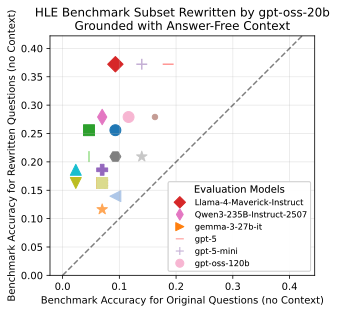
\includegraphics[width=1.0\textwidth]{figs/gpt20b-afc_hle.pdf}
		\caption{Original reference questions.}
		\label{fig:hle-ref-vs-reformat-a}
	\end{subfigure}
	
	\vspace{0.5em} % Adds a small vertical space between the stacked images
	
	% Second Image (b)
	\begin{subfigure}{\columnwidth}
		\centering
		\includegraphics[width=1.0\textwidth]{figs/gpt20b-afc_hle_giveaway.pdf}
		\caption{Reformulated questions generated by model ensemble.}
		\label{fig:hle-ref-vs-reformat-b}
	\end{subfigure}
	
	\caption{Humanities Last Exam (HLE) benchmark evaluation accuracy. Subfigure (a) uses the original reference questions, and Subfigure (b) uses the reformatted questions generated by a model ensemble. This demonstrates reasonable correlation between human and synthetic evaluation.}
	\label{fig:hle-ref-vs-reformat-gpt20}
	\vspace{-1em}
\end{figure*}




\section{Conclusion}

LM-based generative clarification and disambiguation of questions works when the LM is provided relevant context, even if that context does not include the answer to the question. The disambiguation of the question is enough on its own induce the improvement in model response accuracy. 


\newpage
%\bibliographystyle{IEEEtran}
{\small
\bibliography{references}
}

\newpage
\appendix

\section{Impact of Rewrite on Benchmarks}
\label{apx:rewrite_impact}

\Cref{fig:r_minus_q_apx} presents the distribution of accuracy improvement measured as ($\texttt{Rewrite\_Q} - \texttt{Orig\_Q}$) per-evaluation model across all datasets. 
This demonstrates question rewriting broadly improves benchmark accuracy. %the rewritten questions produce broadly improved benchmark performance for all models compared to the original questions.
\begin{figure}[h!]
	\vspace{-0.5em}
	\centering
	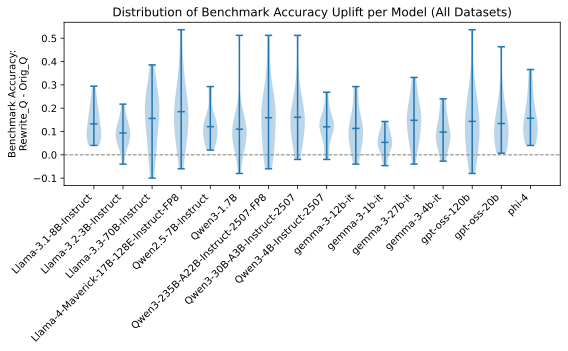
\includegraphics[width=0.9\columnwidth]{figs/acc_uplift_gpt120/r_minus_q.pdf}
	\vspace{-0.8em}
	\caption{Per-dataset per-model difference in benchmark accuracy between the rewritten question and the original question. The violin plot distribution highlights the range of accuracy deltas over all datasets for each model evaluated. Benchmark accuracy improved by an average of 0.1303.}
	\label{fig:r_minus_q_apx}
	% \vspace{-1em}   
\end{figure}
\FloatBarrier

\Cref{fig:r_minus_q_dataset_apx} presents the distribution of accuracy improvement measured as ($\texttt{Rewrite\_Q} - \texttt{Orig\_Q}$) per-dataset instead of per-model like \Cref{fig:r_minus_q_apx}.
\begin{figure}[h!]
	\vspace{-0.5em}
	\centering
	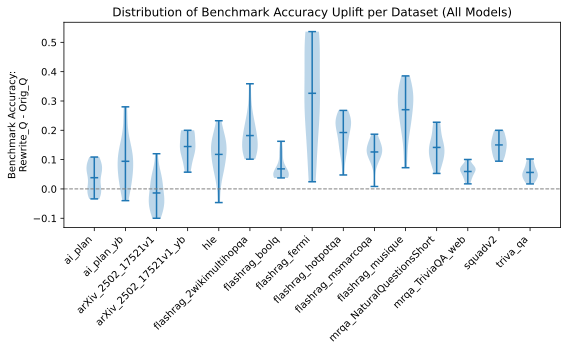
\includegraphics[width=0.9\columnwidth]{figs/acc_uplift_gpt120/r_minus_q_dataset.pdf}
	\vspace{-0.8em}
	\caption{Per-dataset per-model difference in benchmark accuracy between the rewritten question and the original question. The violin plot distribution highlights the range of accuracy deltas over all datasets for each model evaluated. Benchmark accuracy improved by an average of 0.1303.}
	\label{fig:r_minus_q_dataset_apx}
	% \vspace{-1em}   
\end{figure}
\FloatBarrier

%The violin plot information in \Cref{fig:r_minus_q} can be visualized using a scatterplot to break out the effects of model and dataset; where the x-axis is the original benchmark accuracy and the y-axis is the rewritten question performance. 
%\Cref{fig:gpt120b-afc} showcases the results from all datasets before model knowledge cutoffs. 
%All dataset and model combinations lie above the $y=x$ line which indicates identical performance between the original and rewritten questions. 
%Some dataset model combinations get more uplift than others, but there are no combinations where benchmark performance decreases. 

\Cref{fig:r_minus_q_afc_giveaway_apx} presents the distribution of accuracy improvement measured as ($\texttt{Rewrite\_Q} - \texttt{Orig\_Q+AFC}$) per-evaluation model across all datasets. 
\begin{figure}[h!]
	\vspace{-0.5em}
	\centering
	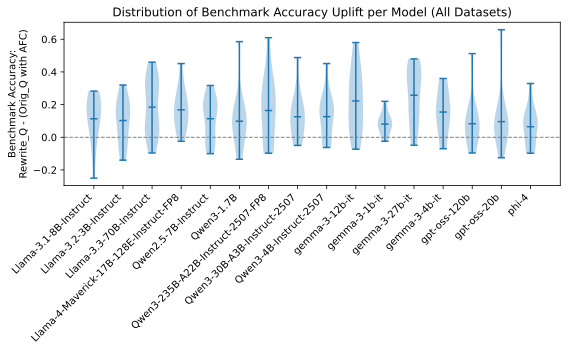
\includegraphics[width=0.9\columnwidth]{figs/acc_uplift_gpt120/rafc_minus_qafc_giveaway.pdf}
	\vspace{-0.8em}
	\caption{Per-model difference in benchmark accuracy between the rewritten questions and the original questions with associated answer-free context. The violin plot distribution highlights the range of accuracy deltas over all datasets for each model evaluated. Benchmark accuracy improved by an average of 0.1346.}
	\label{fig:r_minus_q_afc_giveaway_apx}
	% \vspace{-1em}   
\end{figure}
\FloatBarrier

\Cref{fig:r_minus_q_afc_giveaway_dataset_apx} presents the same information as \Cref{fig:r_minus_q_afc_giveaway_apx}, but with each violin distribution per-dataset instead of per-model.
\begin{figure}[h!]
	\vspace{-0.5em}
	\centering
	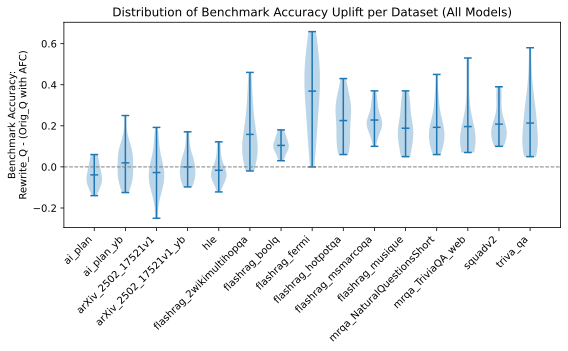
\includegraphics[width=0.9\columnwidth]{figs/acc_uplift_gpt120/rafc_minus_qafc_giveaway_dataset.pdf}
	\vspace{-0.8em}
	\caption{Per-dataset per-model difference in benchmark accuracy between the rewritten questions and the original questions with associated answer-free context. The violin plot distribution highlights the range of accuracy deltas over all models for each dataset evaluated. Benchmark accuracy improved by an average of 0.1346.}
	\label{fig:r_minus_q_afc_giveaway_dataset_apx}
	% \vspace{-1em}   
\end{figure}
\FloatBarrier

\Cref{fig:rafc_giveaway_minus_qafc_giveaway_dataset_apx} demonstrates the benchmark accuracy distribution per-dataset of \texttt{Rewrite\_Q+AFC - Orig\_Q+AFC}.
This combination limits the potential accuracy improvement but reduces the number of datasets which show no average improvement in accuracy.
This may indicate that disambiguation and context inclusion are complementary.
\begin{figure}[h!]
	\vspace{-0.5em}
	\centering
	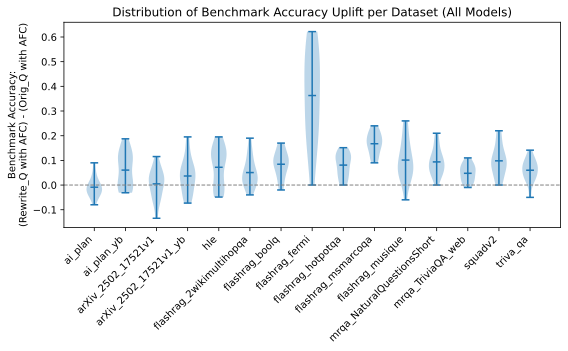
\includegraphics[width=0.9\columnwidth]{figs/acc_uplift_gpt120/rafc_giveaway_minus_qafc_giveaway_dataset.pdf}
	\vspace{-0.8em}
	\caption{Per-dataset improvement in benchmark accuracy from \texttt{Rewrite\_Q} with \texttt{AFC} compared to the \texttt{Orig\_Q} with \texttt{AFC} during benchmark evaluation. Benchmark accuracy improved by an average of 0.0875.}
	\label{fig:rafc_giveaway_minus_qafc_giveaway_dataset_apx}
	%	\vspace{-1em}   
\end{figure}
\FloatBarrier








\section{Question Rewriting Prompt}
\label{apx:rewrite-prompt}

{\scriptsize % \footnotesize
	\begin{lstlisting}[language=json]
		QUESTION_REFORMAT_PROMPT = """
		## Your Role
		
		You are an expert educational content creator specializing in editing and improving evaluation questions to determine the competency of domain experts based on the provided textual information. 
		
		## Input Structure
		
		Your input consists of:
		
		<question>
		[A question to be answered.]
		</question>
		
		<answer>
		[The correct answer to the question.]
		</answer>
		
		<context>
		[The text segment containing information relevant to the question.]
		</context>
		
		## Primary Objective
		
		Your goal is to reformat, rephrase, and rewrite the question according to the provided instructions. The rewritten question should be semantically equivalent to the original question, rewritten for clarity while preserving the same correct answer. This should only be accomplished by filling in background information and explicitly stating assumptions. You are creating a test/quiz question, so DO NOT include the answer information in the question, as that would be a giveaway which skews the results. NEVER include the answer or information which would give away the answer in the rewritten question.
		
		## Analysis Phase
		
		Conduct careful analysis within `<document_analysis>` tags, following these steps:
		
		1. **Thoughtful Content Examination**
		- Carefully analyze the given context, question, and answer; identifying central ideas, nuanced themes, and significant relationships within it.
		
		2. **Concept Exploration**
		- Consider implicit assumptions, subtle details, underlying theories, and potential applications of the provided information.
		
		3. **Intentional Question Planning**
		- Plan how the question can invite deeper understanding, meaningful reflection, or critical engagement, ensuring the question is purposeful.
		
		4. **Detailed Assumption Expansion**
		- Consider what knowledge the question is asking about, and what information and assumptions have been made when formatting the question. Your goal is to provide all the background information and explicitly state assumptions to enhance the clarity of the question.
		
		5. **Giving Away the Answer**
		- Plan how to avoid giving away the answer in the rewritten question. 
		- NEVER include the answer or information which would give away the answer in the rewritten question.
		
		### Documentation in Analysis:
		
		- Clearly document the rationale in the `<document_analysis>` tags, explaining your reasons for exclusion or inclusion decisions.
		- Clearly document what elements of the question need to be disambiguated. What steps need to be taken and what information needs to be include most clearly and concisely disambiguate the question. 
		- Clearly document what information needs to be avoided in the rewritten question to prevent giving away the answer. For example if the question asks about what year a person was born, the question should not include birthday in the biographical details.
		
		
		## Question Rewriting Guidelines
		
		### Encouraged Question Characteristics:
		
		- **Thoughtful Engagement**: Prioritize creating questions that inspire deeper thought and nuanced consideration.
		- **Deep Understanding and Insight**: Ensure that the question and answers require a deep understanding of the content by a professional domain expert.
		- **Self-contained Clarity**: Questions and answers should contain sufficient context, clearly understandable independently of external references.
		- **Brevity**: The rewritten question should be as short as is reasonable while still being clear, understandable, self-contained, and unambiguous.
		
		### Permitted Question Types:
		
		- Analytical
		- Application-based
		- Clarification
		- Counterfactual
		- Understanding
		- Conceptual
		- Factual
		- Open-ended
		- False-premise
		- Edge-case
		- Inference
		- Implication
		- Prediction
		
		(You do not need to use every question type, only those naturally fitting the content and instructions.)
		
		## Output Structure
		
		Present your final output strictly adhering the `<output_format>` tags.
		<output_format>
		Question: [ Question Text ]
		Explanation: [Brief explanation of why the answer is correct]
		Correct Answer: [Short answer]
		</output_format>
		
		## Output
		
		Begin by thoughtfully analyzing the provided context within `<document_analysis>` tags. Then present the resulting formatted question answer pair clearly within `<output_format>` tags.
		
		## Important Notes
		
		- NEVER modify the core element the question is asking about. The knowledge being evaluated shall not change. 
		- Question disambiguation and modification must be grounded in the `<context>`. 
		- Maintain clear, direct, and accurate citations/explanations drawn verbatim from the provided context.
		- Each "thought_process" should reflect careful consideration and reasoning behind your response.
		- When rewriting questions, NEVER include phrases like 'as per the text,' 'according to the document,' or any similar explicit references. Questions should inherently integrate content naturally and stand independently without explicit references to the source material. Make sure that the question is answerable by a domain expert **without the context paragraph**. 
		- Include all relevant context information in the question. Make the question as long and detailed as required so that the test taker can fully understand what is being asked.
		- NEVER include the answer in the rewritten question.
		- Ensure rigorous adherence to output formatting and generate a single `<output_format>` tag block.
		- Verify that the correct answer is in fact correct and the best version of that answer.
		- Verify that the question and answer are semantically equivalent to the original question and answer.
		
		
		
		<question>{question}</question>
		<answer>{answer}</answer>
		<context>{context}</context>
		"""
	\end{lstlisting}
}





\section{Answer-Free Context Creation}
\label{apx:afc}

{\scriptsize % \footnotesize
	\begin{lstlisting}[language=json]
		ANSWER_FREE_CONTEXT_PROMPT = """
		## Your Role
		
		You are an expert educational content creator specializing in editing and improving evaluation questions to determine the competency of domain experts based on the provided textual information. 
		
		## Input Structure
		
		Your input consists of:
		
		<question>
		[A question to be answered.]
		</question>
		
		<answer>
		[The correct answer to the question.]
		</answer>
		
		<context>
		[The text segment containing information relevant to the question.]
		</context>
		
		## Primary Objective
		
		Your goal is to reformat, rephrase, and rewrite the context information according to the provided instructions. The rewritten context should be minimally modified, and semantically equivalent to the original context. The rewrite should only remove the information which gives away the answer to the question. You are creating background material for a test/quiz question, so you need to COMPLETLELY remove the information which gives away the answer to the question from the context. NEVER include the answer or information which would give away the answer in the rewritten context.
		
		## Analysis Phase
		
		Conduct careful analysis within `<document_analysis>` tags, following these steps:
		
		1. **Thoughtful Content Examination**
		- Carefully analyze the given context, question, and answer; identifying central ideas, nuanced themes, and significant relationships within it.
		
		2. **Concept Exploration**
		- Consider implicit assumptions, subtle details, underlying theories, and potential applications of the provided information.
		
		3. **Intentional Context Planning**
		- Plan how the context information can support disambiguation of the question, while not giving away the answer; ensuring the question is purposeful.
		
		4. **Detailed Assumption Expansion**
		- Consider what knowledge the question is asking about, and what information and assumptions have been made when formatting the question. Your goal is to edit the context to remove the information which would give the questions answer away to the test taker.
		
		5. **Giving Away the Answer**
		- Plan how to avoid giving away the answer in the rewritten context. 
		- Figure out what minimal set of information needs to be removed to avoid giving away the answer.
		- NEVER include the answer or information which would give away the answer in the rewritten context.
		
		### Documentation in Analysis:
		
		- Clearly document the rationale in the `<document_analysis>` tags, explaining your reasons for exclusion or inclusion decisions.
		- Clearly document what elements of the context need to be modified. What steps need to be taken and what information needs to be include most clearly and concisely (with minimal modification) remove the answer information from the context. 
		- Clearly document what information needs to be avoided in the rewritten context to prevent giving away the answer. For example if the question asks about what year a person was born, the context should not include birthday in the biographical details.
		
		
		## Context Rewriting Guidelines
		
		## Output Structure
		
		Present your final output strictly adhering the `<output_format>` tags.
		<output_format>
		[ Rewritten Context ]
		</output_format>
		
		## Output
		
		Begin by thoughtfully analyzing the provided question, answer and context within `<document_analysis>` tags. Then present the resulting edited context within `<output_format>` tags.
		
		## Important Notes
		
		- NEVER modify what the question is asking about. NEVER modify the answer. The knowledge being evaluated SHALL NOT change. 
		- Each "thought_process" should reflect careful consideration and reasoning behind your response.
		- NEVER include the answer in the rewritten context.
		- ONLY minimally modify the context as required to remove the answer information. The modified context should be as similar to the original as possible, with the answer information removed. 
		- ONLY remove answer information, do not add new information, and do not remove extraneous information.
		- Ensure rigorous adherence to output formatting and generate a single `<output_format>` tag block.
		
		
		
		<question>{question}</question>
		<answer>{answer}</answer>
		<context>{context}</context>
		"""
	\end{lstlisting}
}



\section{Answer Explanation Validation Prompt}
\label{apx:answer_validation}

{\scriptsize % \footnotesize
	\begin{lstlisting}[language=json]
		EXPLANATION_VALIDATION_PROMPT = """
		## Your Role
		
		You are an expert evaluator of educational content. Your goal is to produce meaningful, insightful knowledge about domain expert evaluations designed to determine competence and knowledge. 
		
		## Input Structure
		
		Your input consists of:
		
		<question>
		[A question to be answered.]
		</question>
		
		<answer>
		[The student's answer to the question.]
		</answer>
		
		<explanation>
		[An explanation for why the answer is correct.]
		</explanation>
		
		<context>
		[The text segment containing information relevant to the question.]
		</context>
		
		## Primary Objective
		
		You will be evaluating and judging the whether the student's answer and their explanation of why their answer is correct makes sense and is logically valid.
		
		Your goal is to judge whether the information presented in `<answer>` is in fact the correct answer to the `<question>` given the information in the `<context>` and whether the `<explanation>` for why the answer is correct is valid. The information in `<context>` and `<question>` can be assumed true, only the context of `<answer>` needs to be validated for correctness.
		
		### Metrics
		
		1. **Answer Correctness:** Rate from 1 to 10 how correct the provided student answer is given the information in the `<question>` and `<context>`. A rating of 1 indicates the answer is incorrect. A rating of 10 indicates the answer is correct and complete. 
		
		2. **Explanation Validity:** Rate from 1 to 10 how valid the students `<explanation>` of their answer is. The `<explanation>` should explain their thinking and the information used to determine the correct answer given the context and question. Low ratings indicate the explanation is not valid, correct, or that there is some flaw in the thinking or logic of the student. High ratings indicate the explanation is valid, correct, and explains why the answer is what it is. 
		
		## Analysis Phase
		
		Conduct careful analysis within `<document_analysis>` tags, following these steps:
		
		1. **Thoughtful Content Examination**
		- Carefully analyze the given context, identifying central ideas, nuanced themes, and significant relationships within it.
		
		2. **Concept Exploration**
		- Consider implicit assumptions, subtle details, underlying theories, and potential applications of the provided information.
		
		## Output Structure
		
		Present your final output strictly adhering the `<output_format>` tags.
		<output_format>
		Answer Correctness: [ Correctness Rating. Respond with a number in [1, 2, 3, 4, 5, 6, 7, 8, 9, 10] ]
		Explanation Validity: [ Validity Rating. Respond with a number in [1, 2, 3, 4, 5, 6, 7, 8, 9, 10] ]
		</output_format>
		
		## Output
		
		Begin by thoughtfully analyzing the provided context within `<document_analysis>` tags. Then present the resulting formatted question answer pair clearly within `<output_format>` tags.
		
		## Important Notes
		
		- Each "thought_process" should reflect careful consideration and reasoning behind your ratings.
		- Ensure rigorous adherence to output formatting.
		
		
		<question>{question}</question>
		<answer>{answer}</answer>
		<explanation>{explanation}</explanation>
		<context>{context}</context>
		"""
	\end{lstlisting}
}



\section{Question Property Validation Prompt}
\label{apx:question_validation}

{\scriptsize % \footnotesize
	\begin{lstlisting}[language=json]
		PROPERTIES_PROMPT = """
		## Your Role
		
		You are an expert evaluator of educational content. Your goal is to produce meaningful, insightful knowledge about domain expert evaluations designed to determine competence and knowledge. 
		
		## Input Structure
		
		Your input consists of:
		
		<question>
		[A question to be answered.]
		</question>
		
		<answer>
		[The correct answer to the question.]
		</answer>
		
		<context>
		[The text segment containing information relevant to the question.]
		</context>
		
		## Primary Objective
		
		You will be evaluating and judging the quality of test and evaluation questions across a variety of metrics. Your goal is to judge and evaluate the quality of various test and evaluation questions across a variety of metrics. The `<question>` and `<answer>` pair is grounded and drawn from the `<context>`. 
		
		### Metrics
		
		1. **Clarity:** Rate from 1 to 10 the clarity and comprehensibility (how understandable it is) of the provided `<question>`. A rating of 1 is unclear and cannot be understood or cannot be understood without the `<context>`. A rating of 10 is used for questions that are self contained, understandable, and coherent (even if the topic is complex and difficult). Questions that are missing information required to understand what is being asked rate a 1. "As of the 2015 NFL season, how many Super Bowl titles had the Denver Broncos won?" is a 10. "What event in 1861 contributed to the temporary strength of republicanism in Britain during Queen Victoria's reign?" is a 10. "In which year was the country not a member of FIFA, as indicated in the table?" is a 1. "As of the census of 2000, how many families were residing in the city?" is a 1.
		
		2. **Difficulty:** Rate form 1 to 10 the difficulty of the `<question>`. A rating of 10 is reserved for questions which require a deep understanding of the question and what is being asked by a professional domain expert. 
		
		3. **Groundedness:** Rate form 1 to 10 how grounded the provided `<question>` is in the `<context>`. A rating of 10 requires the question and answer information can found within the `<context>`. A rating of 1 indicates the question and answer information is not present in the `<context>`. This metric is only concerned with information found in the `<context>`, not outside information. The more outside information (not contained in the `<context>`) that is required to answer the question, the lower the rating.
		
		4. **Answer Give Away:** Rate from 1 to 10 how much the provided `<answer>` is given away by information in the `<question>`. A rating of 1 indicates that the information requried to answer the question is not present in the question itself. A rating of 10 indicates that the information required to answer the question is present in the question.
		
		## Analysis Phase
		
		Conduct careful analysis within `<document_analysis>` tags, following these steps:
		
		1. **Thoughtful Content Examination**
		- Carefully analyze the given context, identifying central ideas, nuanced themes, and significant relationships within it.
		
		2. **Concept Exploration**
		- Consider implicit assumptions, subtle details, underlying theories, and potential applications of the provided information.
		
		## Output Structure
		
		Present your final output strictly adhering the `<output_format>` tags.
		<output_format>
		Clarity: [ Clarity Rating (one of [1, 2, 3, 4, 5, 6, 7, 8, 9, 10] ) ]
		Difficulty: [ Difficulty Rating (one of [1, 2, 3, 4, 5, 6, 7, 8, 9, 10] ) ]
		Groundedness: [ Groundedness Rating (one of [1, 2, 3, 4, 5, 6, 7, 8, 9, 10] ) ]
		Answer Giveaway: [ Answer Giveaway Rating (one of [1, 2, 3, 4, 5, 6, 7, 8, 9, 10] ) ]
		</output_format>
		
		## Output
		
		Begin by thoughtfully analyzing the provided context within `<document_analysis>` tags. Then present the resulting formatted question answer pair clearly within `<output_format>` tags.
		
		## Important Notes
		
		- Each "thought_process" should reflect careful consideration and reasoning behind your ratings.
		- Ensure rigorous adherence to output formatting.
		
		
		<question>{question}</question>
		<answer>{answer}</answer>
		<context>{context}</context>
		"""
	\end{lstlisting}
}


\end{document}
